\chapter{Engine architecture overview}

Now, after the last chapter described many different kinds and sizes of engines, this section is going to examine the architecture that powers an engine. At the beginning an overview of a modern game engine's runtime architecture is given. That overview is then followed by a description of several selected submodules. These power different systems of the engine and are responsible for its performance and functionality. The submodules were chosen based on the author's opinion of their relevance and importance to the backbone of an engine.

\section{General runtime architecture}

When talking about software parts of an engine in a high level fashion it can be separated into two clearly diverging parts, tools and the runtime component. This section will almost entirely discuss the runtime part while only mentioning the most important tools at the end. An engine consists from many modules which are separated into different layers. Game engines share this architectural design decision with many other software projects that reach a specific size. Layers group modules together with other ones operating in the same order of magnitude as their siblings. A layer often depends upon lower ones but shall not have any dependencies to upper ones. This ensures that coupling between layers is loose which leads to more stable software solutions. An exemplary illustration of a generic engine's runtime architecture can be seen in Figure \ref{fig:engine_runtime_arch}.

\begin{figure}[h!]
	\centering 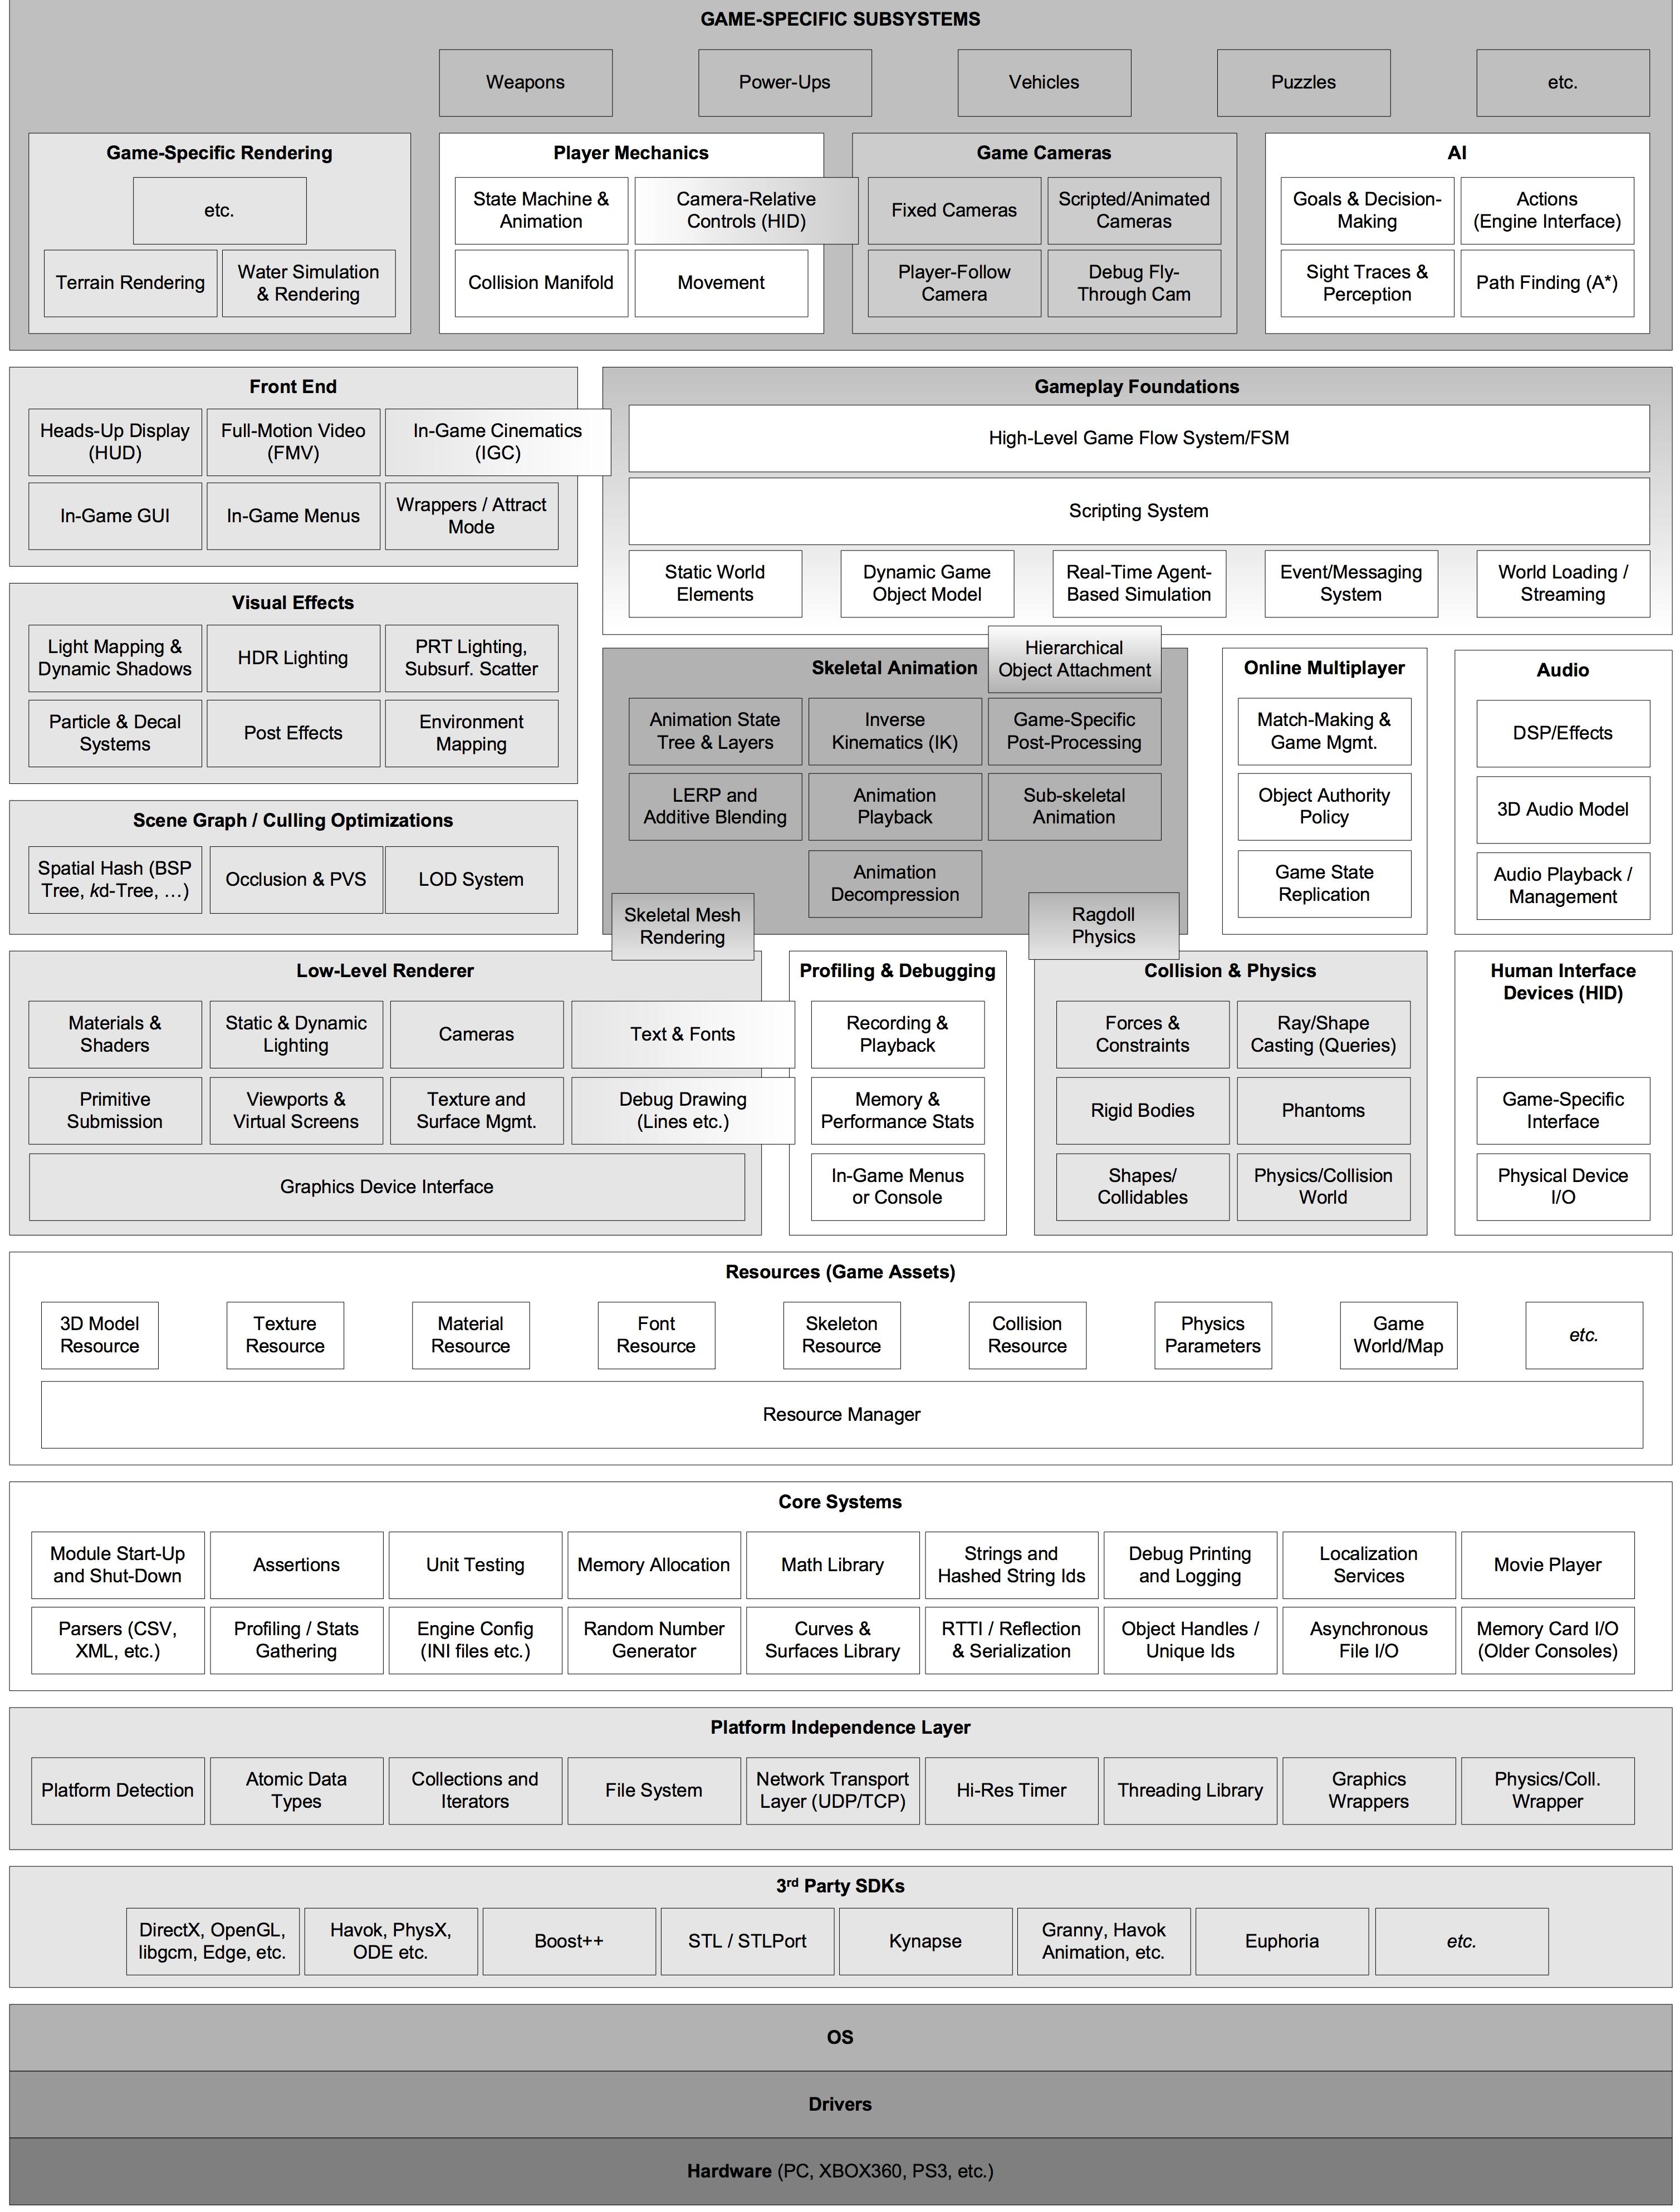
\includegraphics[width=\linewidth]{PICs/engine_runtime_arch.jpg}
	\caption{Illustration showing common modules grouped into distinct layers of a large scale engine solution}
	\label{fig:engine_runtime_arch}
\end{figure}

The complexity of modules in a layer grows when ascending through them from bottom to top. Where the lowermost layers include low-level systems essentially drivers \footnote{A program that controls or communicates with a hardware device}, platform-dependent 3\textsuperscript{rd} party \acp{SDK} or platform-independent abstraction components. Traversing the hierarchy upwards from core systems, over resource management, to general rendering and gameplay foundation modules, at one point the uppermost layers are reached. Those encompass game specific subsystems that can vary from one game to another. With the crude knowledge of the different layers involved in an engine it can be emphasized that a game engine is a highly complex software and building one is an endeavor that requires expertise, experience and time. It is important to properly reason out the architecture and uphold the focus onto the engine's goal. Maintaining focus while following the sketched out architecture will help to avoid unnecessary coupling and the implementation of irrelevant features or systems. 
The rest of this section will describe some modules from Figure \ref{fig:engine_runtime_arch} in-depth to investigate how they work and how they contribute to the combined whole.

\section{Memory Management}

One key constraint nearly every engine has to fulfill is running games with a high frame rate. Because games are real-time simulations the time window for running gameplay logic and rendering a single frame is very limited. To complement this with discrete numbers for a game, running with 60 \ac{FPS} a slice of 16.6 ms can be used per single frame. To stay into this limits game developers came up with optimization techniques and algorithms that speed up calculations and processing. But the performance of code is not only dependent upon the efficiency of an applied algorithm but also how the program manages and uses its resources, especially memory. Controlling how an engine utilizes the \ac{RAM} is mandatory for guaranteeing high performance. The two most commonly applied memory usage optimizations are either reducing the amount of dynamic allocations at a game's runtime or allocating bigger sections of memory to store data in contiguous blocks. To solve these problems engines often implement custom memory allocators that have a better runtime performance then using the existing system allocator.

\subsection{Custom Allocators}
\blindtext

\section{Job System}
\blindtext
\section{Rendering}
\blindtext
\section{Entity Component System}
\blindtext
\section{Scripting}
\blindtext
\section{Tools}
\blindtext
\subsection{Editor}
\blindtext
\subsection{Asset pipeline}
\blindtext